\section{Einführung}
Um solche synthetischen Pflanzenskizzen zu erzeugen, bedient man sich der 
Schraffurtechnik. Durch diese Technik erhält man ein hohes Maß an 
Detailreichtum, Anwendung neben der Erzeugung solcher synthetischer 
Pflanzenskizzen ist auch die Erzeugung synthetischer Kupferstiche, was eine 
seit dem Mittelalter genutzte Technik ist.
\par Grundsätzlich hängt eine solche Schraffur von einigen Parameter an:

\begin{itemize}
  \item von Schatten und Helligkeitsabstufungen im Originalbild
  \item von Objekt- und Materialeigenschaften (Kanten, Falten; Texturen)
  \item von Unterschiedlichen Farben
\end{itemize}

Eine weitere Frage, die man sich stellt ist "`Wie kann man Schraffuren 
variieren?"'

\begin{itemize}
  \item Wo sind Linien?
  \item Länge der Linien
  \item Wie verlaufen sie? In Bezug auf Richtung und Linienart
  \item Parallelität der Linien innerhalb einer Schraffur
  \item Dichte der Linien
\end{itemize}

Das Einsatzgebiet solcher Schraffuren ist vielfältig, man findet diese in 
Bleistiftzeichnungen, bei Linien im NPR-Bereich: detailreiche Karikaturen, 
Bewegungslinien in Cartoons, in Stroke-based Illustrations, bei der Simulation 
von Holzschnitten, Kupferstichen oder eben bei Pflanzenskizzen.

\section{Funktionsweise}
Zuerst wollen wir hier auf die Erzeugung solcher Schraffuren bei synthetischen 
Kupferstichen eingehen, da die Technik grundlegend ist, um auch synthetische 
Pflanzenskizzen erzeugen zu können. Der algorithmische Ansatz zur Herstellung 
solcher Schraffuren interpretiert die Schraffurlinien als Schnitte zwischen der 
darzustellenden dreidimensionalen Geometrie und einer Schar von Ebenen. Andere 
Verfahren verwenden Volumenfunktionen oder Hauptkrümmungsrichtungen. \par Die 
Verwendung von Schnittebenen hat den Vorteil, dass man die Ebenenschar auf eine 
Weise spezifizieren kann, die den Linien ästhetisch ansprechende Formen 
verleihen.
Zusammenfassend lässt sich das Verfahren also wie folgt strukturieren:

\begin{itemize}
  \item Zerlegung des Geometriemodells in einzeln zu schraffierende Teile
  \item pro Teil: Spezifikation einer Ebenenschar mittels graphischem Editor
  \item Berechnung der Schnittlinien der Ebenen
\end{itemize}

Dadurch soll die Form der Schraffurlinien wiedergegeben werden (wie Geometrie, 
Lichtverhältnisse $\to$ Liniendicke). \par Das Ziel bei der Herstellung 
synthetischer Pflanzenskizzen ist die Vermittlung des Eindrucks eines Modells 
einer Landschaft durch Form und Größenverhältnisse, ohne eine konkrete 
Ausprägung zu erreichen. Um beispielsweise eine Baumskizze zu erzeugen, muss 
dieser durch 2 Arten von Geometrie beschrieben werden:

\begin{itemize}
  \item Astwerk mit glatter Oberfläche
  \item Blattwerk aus vielen tausend Einzelflächen
\end{itemize}

Das heißt konkret, dass hier zwei separate Algorithmen zum Einsatz kommen 
müssen, um die Strukturunterschiede erzeugen zu können. Zur Darstellung des 
Baumstamms wird eine ähnliche Technik wie bei Kupferstichen verwendet: Es wird 
die Silhouette gezeichnet und Schraffurstriche an den Stellen, die wenig 
beleuchtet sind. Hierfür wird eine Variante der Halftoning-Methode eingesetzt, 
die diesmal aber keine Punkte, sondern kurze Striche erzeugt. In nachfolgender 
Abbildung \ref{fig:Baum} ist ein Beispiel zu sehen.

\begin{figure}
  \centering
  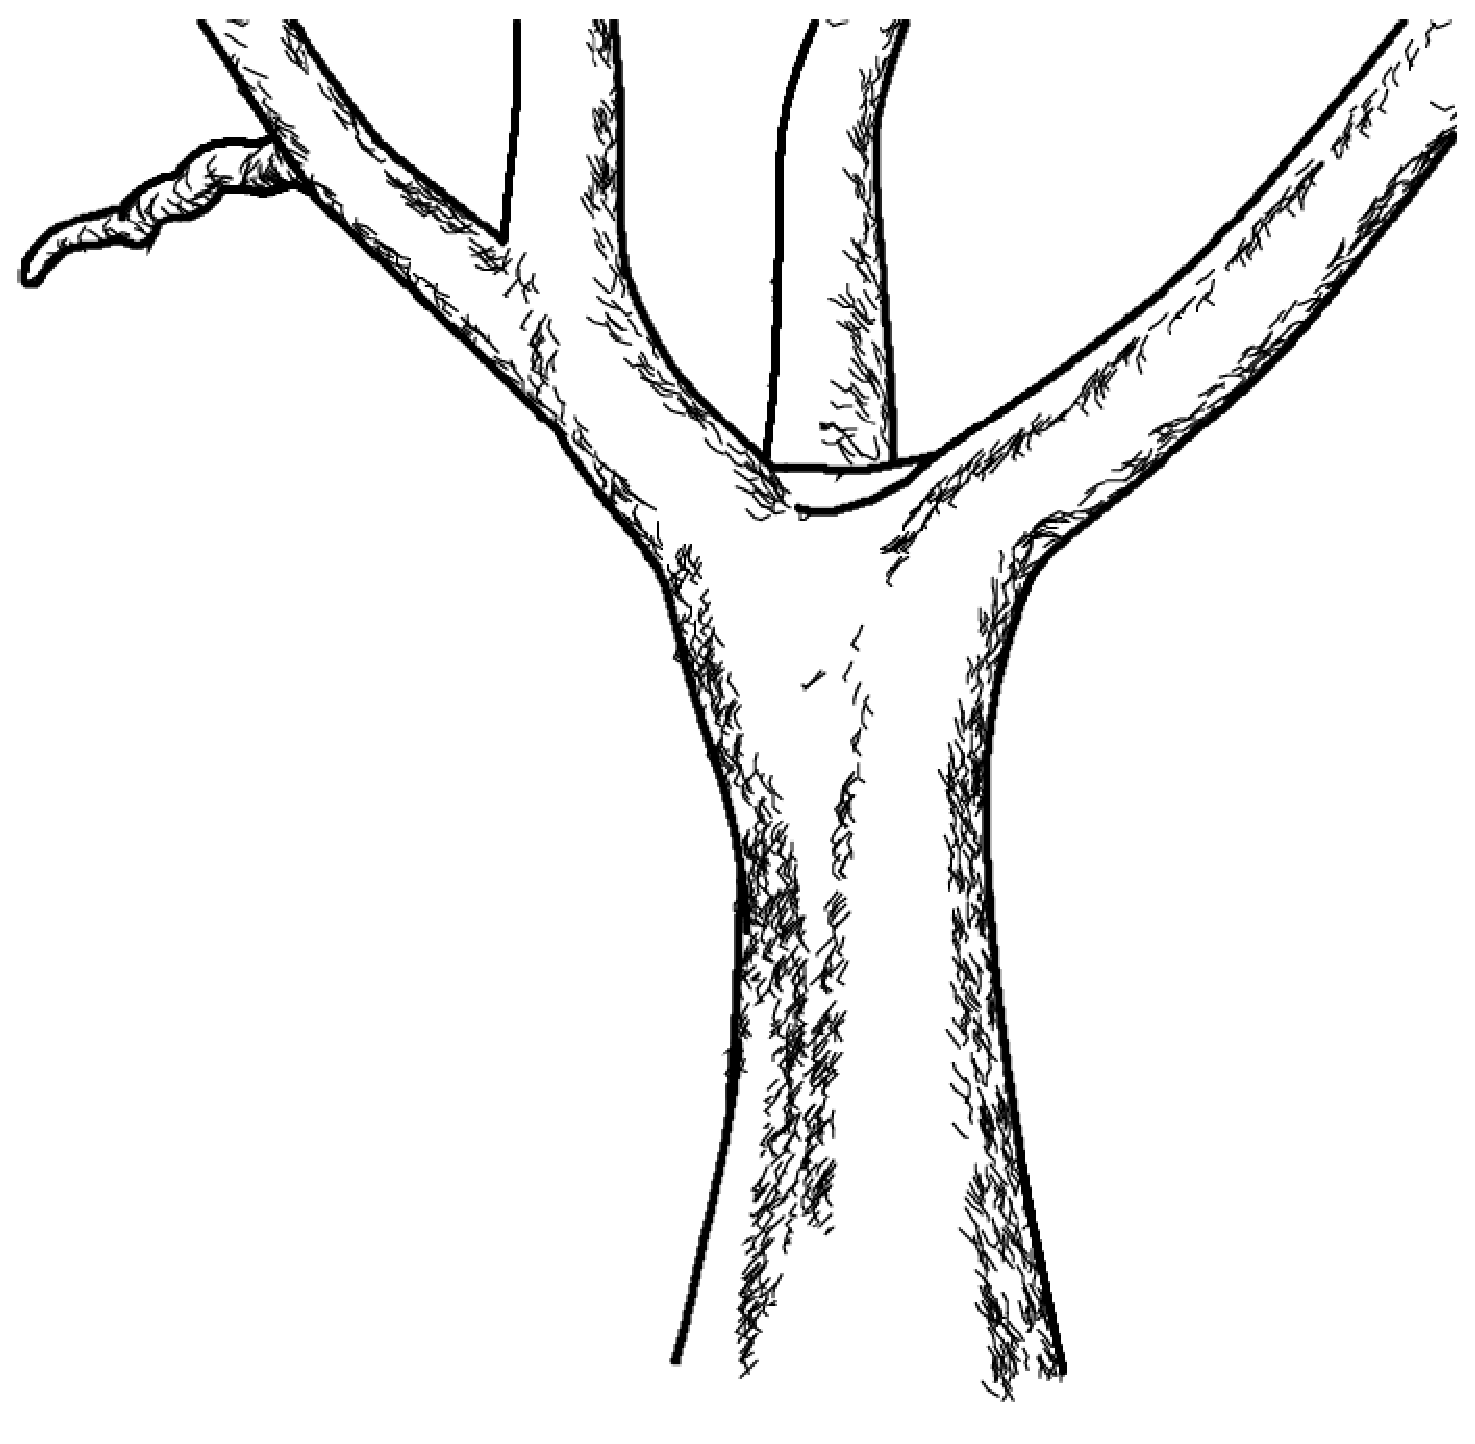
\includegraphics[height=6cm]{../images/Deussen2000-tree-trunk-branches}
  \caption{Stamm und Hauptäste von Baum 1. Quelle: \cite{Deussen2000}.}
  \label{fig:Baum}
\end{figure}

\section{Beispielgrafiken für erzeugte Baumskizzen}
Abschließend sind hier ein paar weitere Beispiele für synthetische Baumskizzen
aufgeführt. Abbildung \ref{fig:baum1-varianten} zeigt dabei den bereits
vorgestellten Baum 1 inkl.\ Blattwerk.

\begin{figure}
  \centering
  \subfloat{
    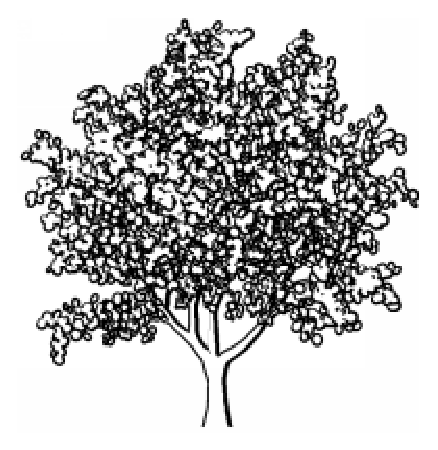
\includegraphics[height=6cm]{../images/Deussen2000-tree1-version1}
  }
  \qquad
  \subfloat{
    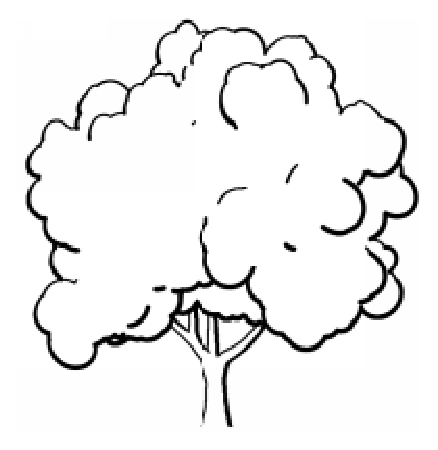
\includegraphics[height=6cm]{../images/Deussen2000-tree1-version2}
  }
  \caption{Baum 1 mit verschiedenen Parametern für Blattwerk und Detailgrad.
  Quelle: \cite{Deussen2000}.}
  \label{fig:baum1-varianten}
\end{figure}

Neben einzelnen Bäumen lässt sich zusätzlich auch die direkte Umgebung eines
Baumes darstellen, wie Abbildung \ref{fig:baum-gross} zeigt.

\begin{figure}
  \centering
  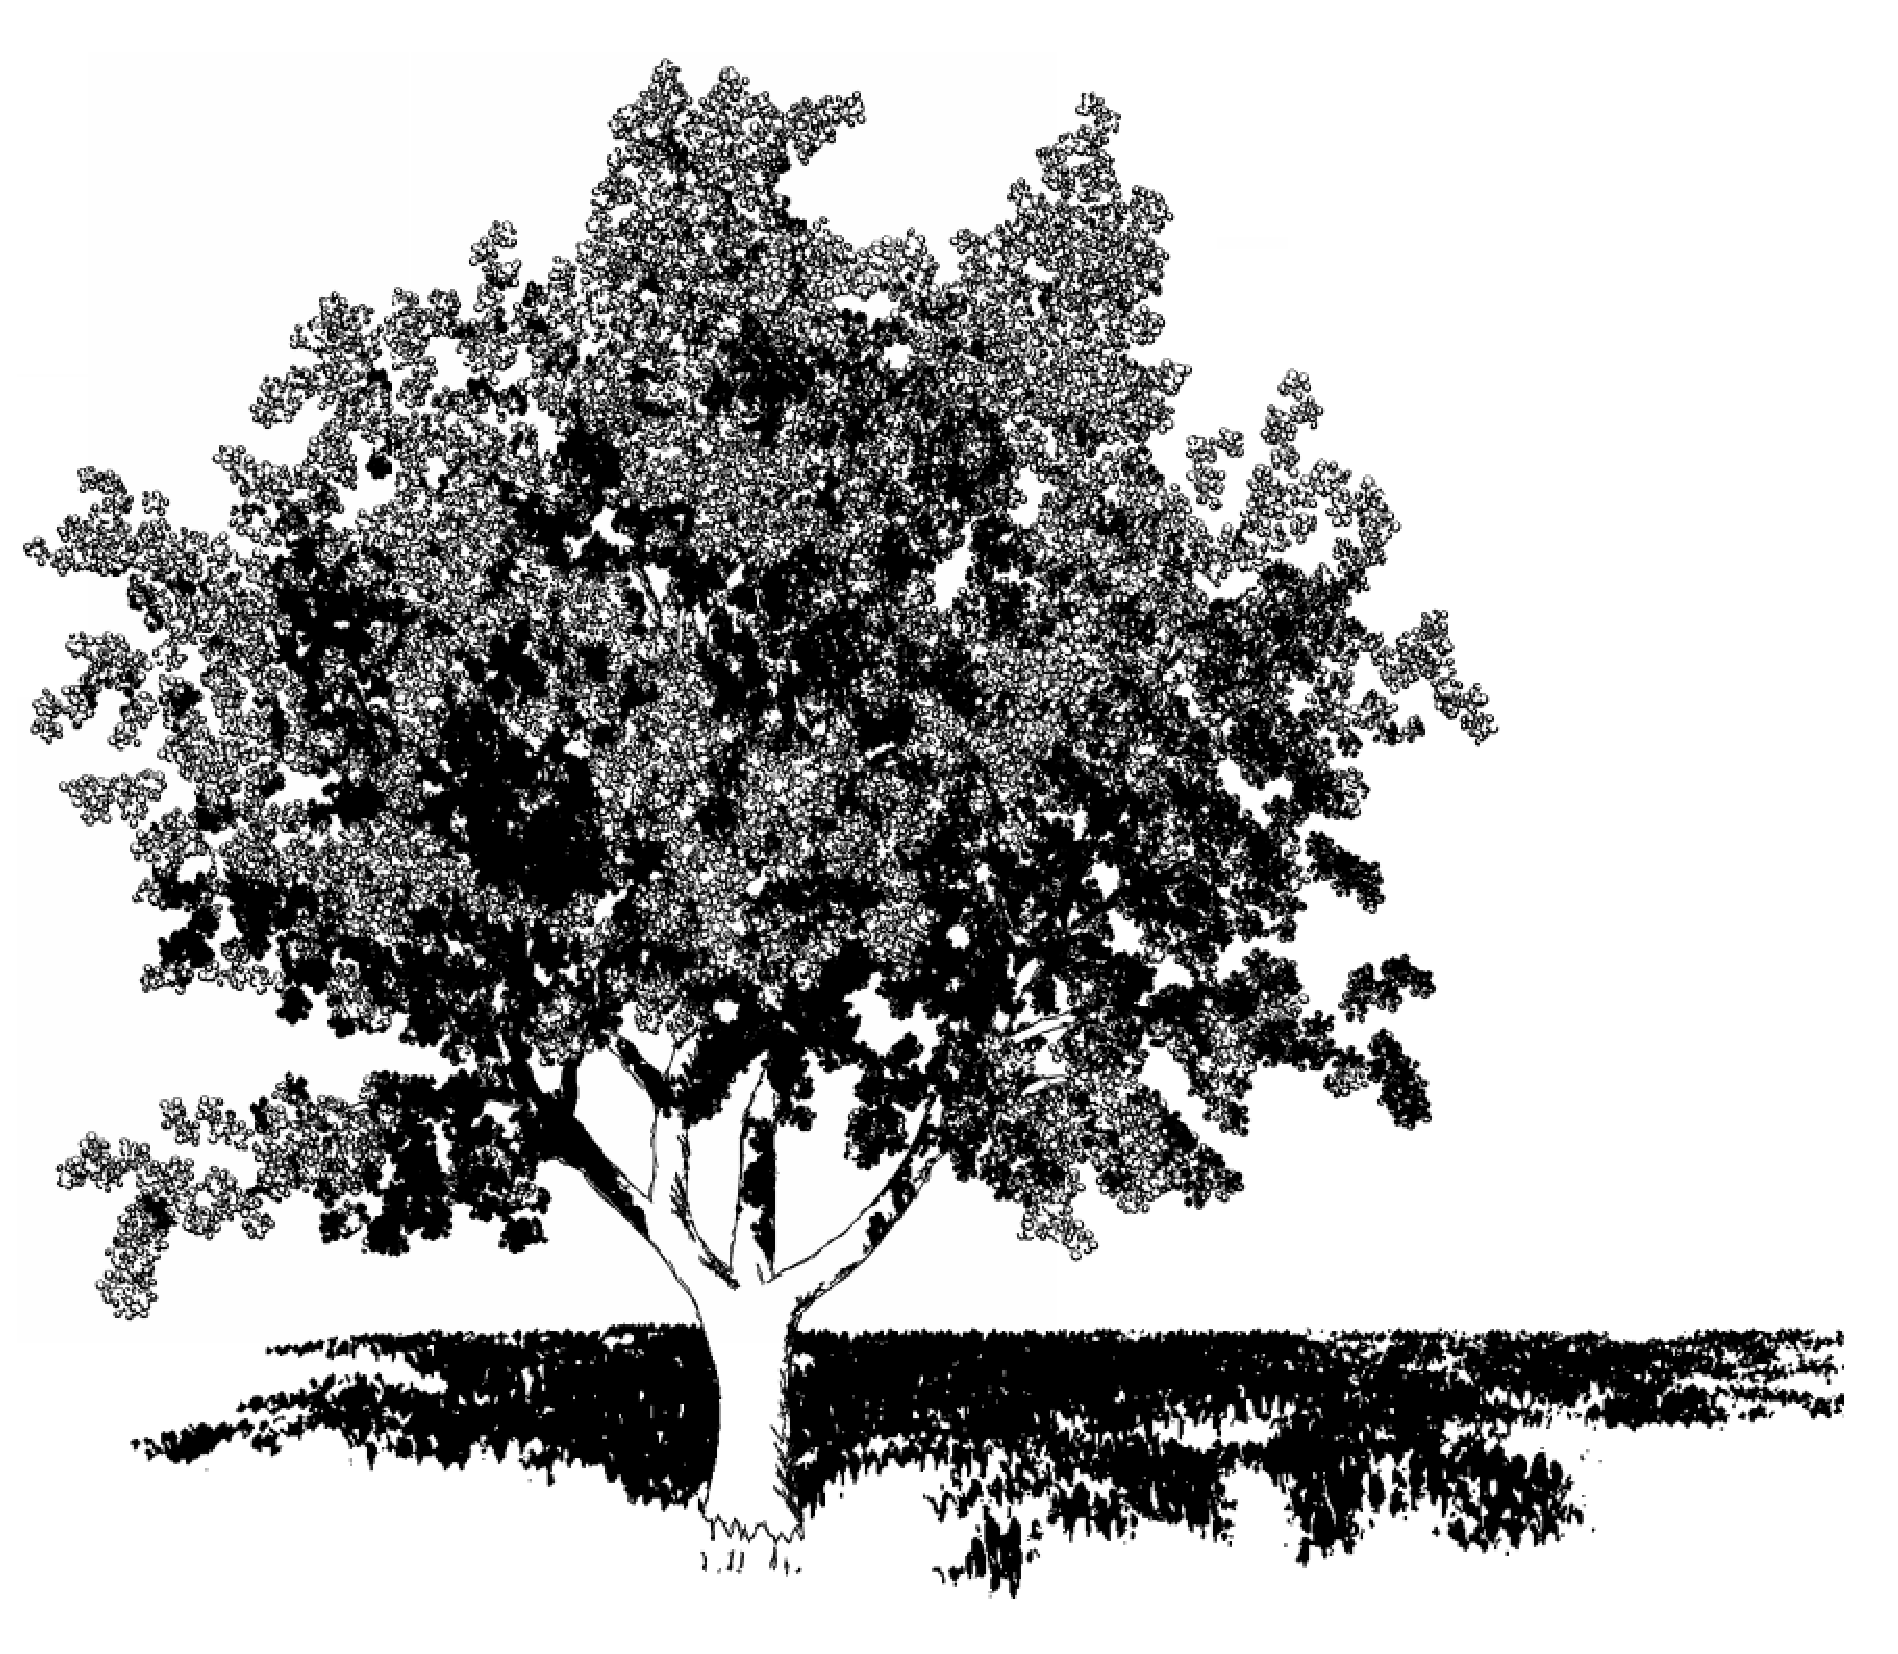
\includegraphics[width=0.8\textwidth]{../images/Deussen2000-tree-large}
  \caption{Baum 3 mit Grasumgebung. Quelle: \cite{Deussen2000}.}
  \label{fig:baum-gross}
\end{figure}